\part{Arithmetic Logic Unit}
\frame{\partpage}

\begin{frame}{Arithmetic Logic Unit}
	\begin{center}
		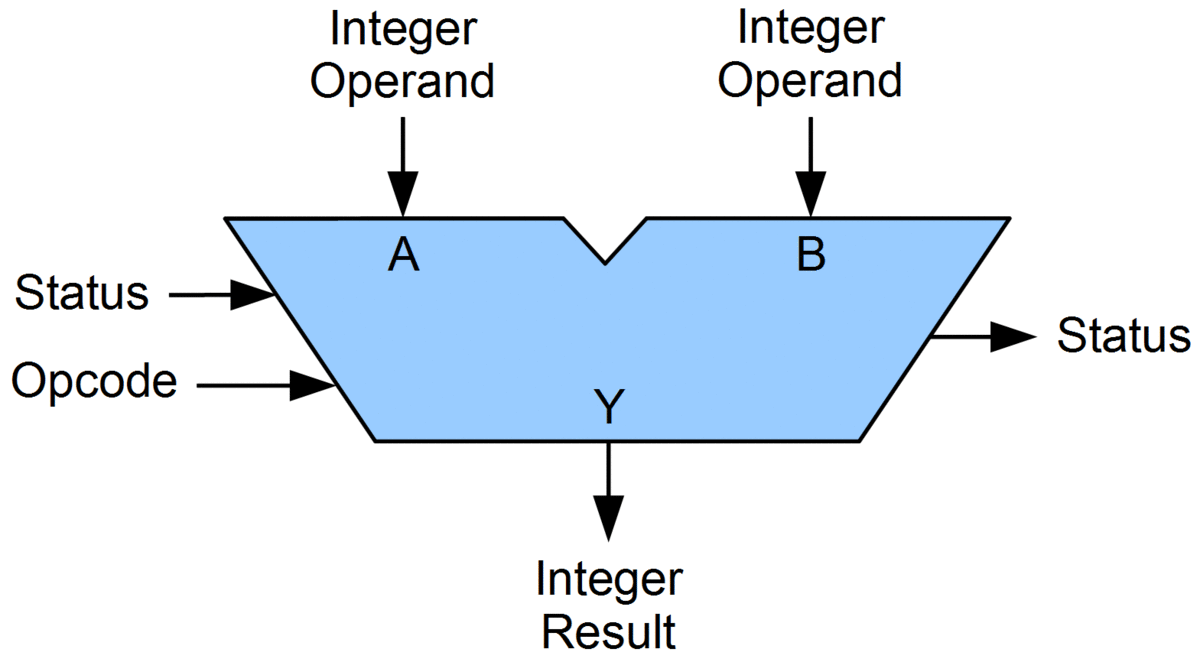
\includegraphics[width=\textwidth]{alu}
		%https://commons.wikimedia.org/wiki/File:ALU_block.gif
	\end{center}
\end{frame}

\begin{frame}{Arithmetic Logic Unit}
	\begin{itemize}
		\pause\item Important part of the CPU
		\pause\item Inputs:
			\begin{itemize}
				\item \textbf{Operand} words $A, B$
				\item \textbf{Opcode}
				\item \textbf{Status} bits
			\end{itemize}
		\pause\item Outputs:
			\begin{itemize}
				\item \textbf{Result} word $Y$
				\item \textbf{Status} bits
			\end{itemize}
		\pause\item Opcode specifies how $Y$ is calculated based on $A$ and $B$
	\end{itemize}
\end{frame}

\begin{frame}{ALU operations}
	Typically include:
	\begin{itemize}
		\pause\item Add with carry
		\pause\item Subtract with borrow
		\pause\item Negate (2's complement)
		\pause\item Increment, decrement
		\pause\item Bitwise \textsc{and}, \textsc{or}, \textsc{not}, $\dots$
		\pause\item Bit shifts
	\end{itemize}
\end{frame}

\begin{frame}{Adding 3 bits}
    \begin{center}
        \begin{tabular}{|ccc|c|}
            \hline
            $A$ & $B$ & $C$ & $A+B+C$ \\\hline
            0 & 0 & 0 & 00 \\
            0 & 0 & 1 & 01 \\
            0 & 1 & 0 & 01 \\
            0 & 1 & 1 & 10 \\
            1 & 0 & 0 & 01 \\
            1 & 0 & 1 & 10 \\
            1 & 1 & 0 & 10 \\
            1 & 1 & 1 & 11 \\\hline
        \end{tabular}
    \end{center}
\end{frame}

\begin{frame}{1-bit adder}
	\begin{center}
		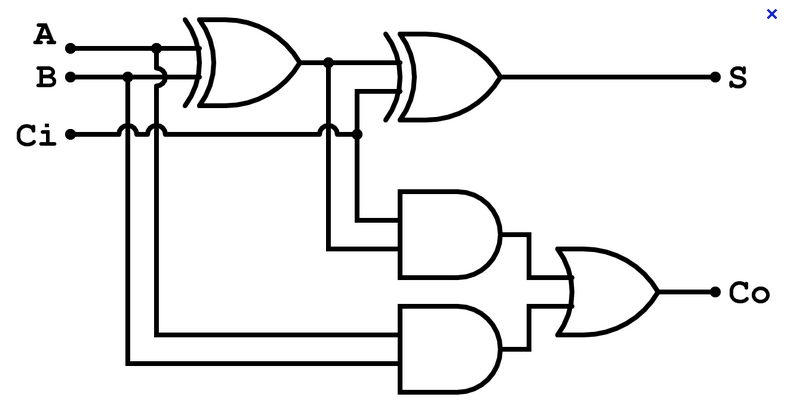
\includegraphics[width=\textwidth]{1bit_adder}
	\end{center}
\end{frame}

\begin{frame}{How does the 1-bit adder work?}
    Exercise:
	\begin{itemize}
		\item Write down the boolean expressions for $S$ and $Co$
		\item Draw a truth table for these
		\item Compare the truth table to the addition table on a previous slide
	\end{itemize}
\end{frame}

\begin{frame}{$n$-bit adder}
	\begin{center}
		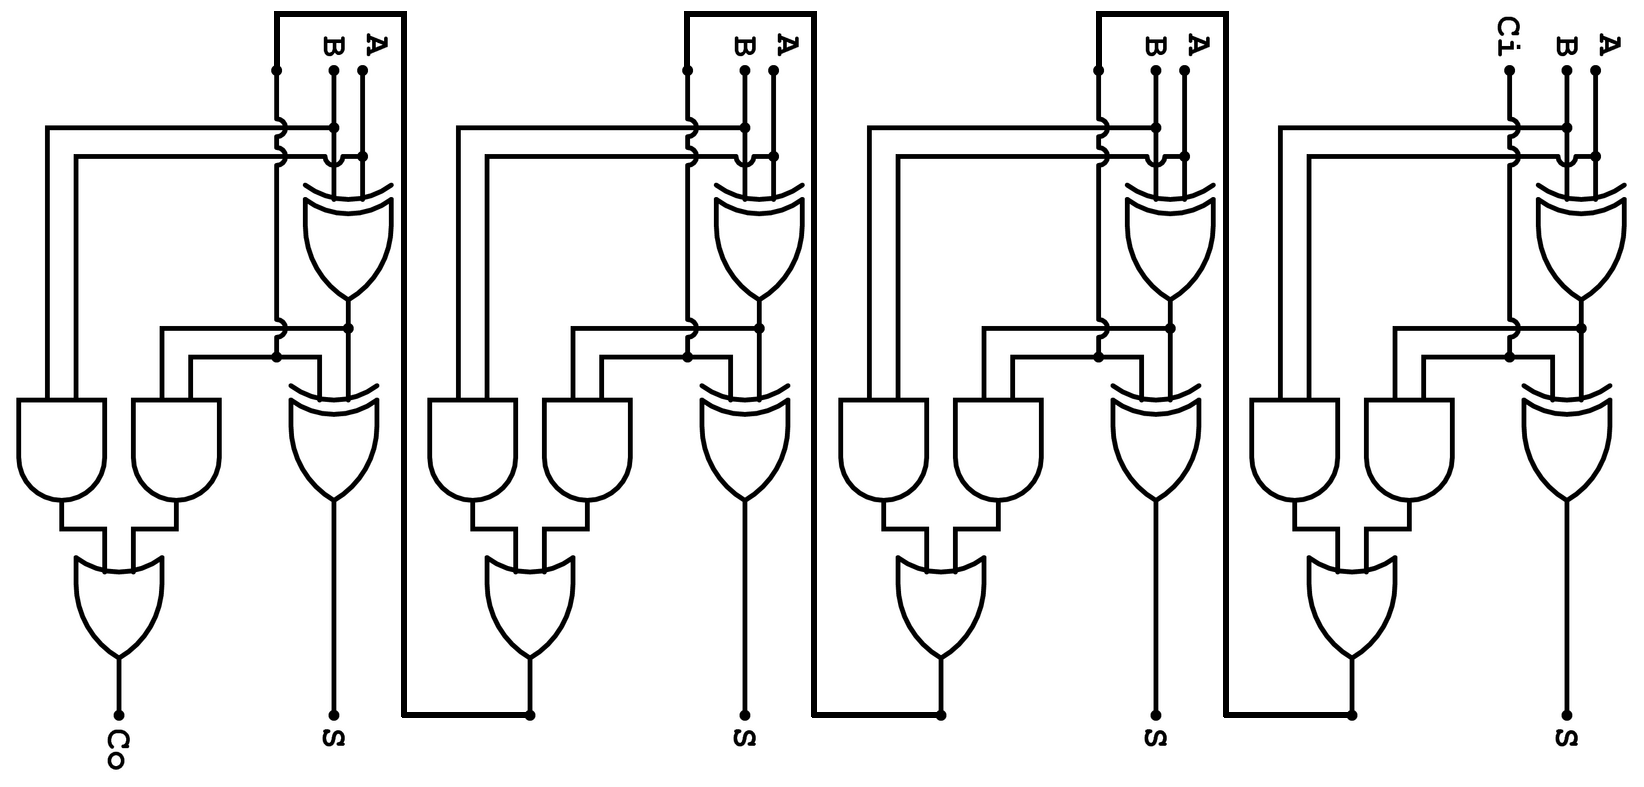
\includegraphics[width=\textwidth]{nbit_adder}
	\end{center}
\end{frame}

